\section{Exceptional fibres and specialization}\label{sec:chambers}

The six chambers have two types of deepest fibre. We first
describe the two-plane fibre, because it shows directly how a
moving exceptional curve acquires two components. We then
calculate the remaining chambers. These finite configurations
occur in Bielawski--Dancer \cite[Example~6.10]{bielawskidancer}.
Section~\ref{sec:compact-interaction} identifies them with the
\emph{whole} fibres in our compact bundle moduli spaces.

\begin{figure}[tb]
\centering
\begin{adjustbox}{max width=\textwidth}
% The parameter plane is zeta_0+zeta_1+zeta_2=0.
% This drawing uses zeta_0=x, zeta_1=-x/2-sqrt(3)y/2,
% zeta_2=-x/2+sqrt(3)y/2. It is not the (s,t) coordinate plane.
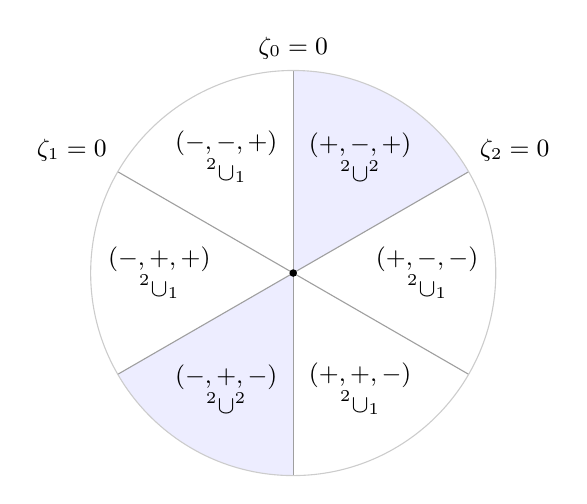
\begin{tikzpicture}[scale=1.05,font=\small]
 \fill[blue!7] (0,0)--(30:2.45) arc(30:90:2.45)--cycle;
 \fill[blue!7] (0,0)--(210:2.45) arc(210:270:2.45)--cycle;
 \foreach \angle in {30,90,150}
  {\draw[gray!75] (\angle:2.45)--(\angle+180:2.45);}
 \draw[gray!40] (0,0) circle[radius=2.45];
 \fill (0,0) circle[radius=1.3pt];
 \node[align=center] at (0:1.62) {$(+,-,-)$\\$\PP^2\cup\FF_1$};
 \node[align=center] at (60:1.62) {$(+,-,+)$\\$\PP^2\cup\PP^2$};
 \node[align=center] at (120:1.62) {$(-,-,+)$\\$\PP^2\cup\FF_1$};
 \node[align=center] at (180:1.62) {$(-,+,+)$\\$\PP^2\cup\FF_1$};
 \node[align=center] at (240:1.62) {$(-,+,-)$\\$\PP^2\cup\PP^2$};
 \node[align=center] at (300:1.62) {$(+,+,-)$\\$\PP^2\cup\FF_1$};
 \node[above] at (90:2.47) {$\zeta_0=0$};
 \node[above right] at (30:2.47) {$\zeta_2=0$};
 \node[above left] at (150:2.47) {$\zeta_1=0$};
\end{tikzpicture}

\end{adjustbox}
\caption{The six sectors in the moment parameter plane. Signs are
ordered $(\zeta_0,\zeta_1,\zeta_2)$. The shaded sectors have
two planes meeting at a point; in the other sectors the two
surfaces meet along a projective line.}
\label{fig:chambers}
\end{figure}

\subsection{Two planes and a reduced degeneration of curves}
Take $\zeta_0=a>0$, $\zeta_2=b>0$, and $\zeta_1=-a-b$.
Over the affine vertex every oriented-cycle invariant vanishes.
In particular,
\[
 zz'=ww'=0,\qquad u_i\varphi_j=0\quad(1\le i,j\le2).
\]
Thus $u=0$ or $\varphi=0$, and a nonzero triangle of
arrows must be acyclic. If $\varphi\ne0$, the positive
moment at vertex~2 forces $w\ne0$; the cycle equations
then force $z'=w'=0$. This component, including its
closure, is
\begin{equation}\label{eq:plane-zero-section}
 u=z'=w'=0,\qquad |z|^2+|\varphi|^2=a,\qquad
 |w|^2=b+|\varphi|^2.
\end{equation}
Eliminate the nonzero coordinate $w$ by complex gauge.
The remaining quotient is $[z:\varphi]\in\PP^2$.
Call it $P_0$: its objects have $L_0$ as subobject
and the spherical extension of $L_1,L_2$ as quotient.
The other component $P_2$ has $\varphi=z'=w'=0$,
$z\ne0$, and coordinates $[w:u]\in\PP^2$.
The components meet at the single point $p$ with
$u=\varphi=0$ and $z,w\ne0$.

These are all the components, since they exhaust the
acyclic supports. Near $p$ fix $z,w$ by complex gauge
and solve the two complex equations for $z',w'$.
The remaining smooth coordinates are $(u,\varphi)$.
Thus $P_0=\{u=0\}$ and $P_2=\{\varphi=0\}$ meet
transversely. The moving exceptional divisor $D$ is
locally $\varphi(u)=0$, with contraction to the
$A_1$ surface given by
\[
 A=u\otimes\varphi,\qquad \tr A=0.
\]
In particular, $D$ has an ordinary double point at $p$.
It is irreducible: its projective-line family over the
connected open surface $S^\circ$ is dense, and a
fibre over $o$ has dimension two, not three.

Fix nonzero $b_0\in\C^2$ and
$\beta_0\in(\C^2)^*$ with $\beta_0(b_0)=0$.
Over $A=t b_0\otimes\beta_0$, write
$u=\lambda b_0$, $\varphi=\nu\beta_0$,
$\lambda\nu=t$, and $z'=w'=0$. The compact
quotient has coordinates
\begin{equation}\label{eq:proper-specialization}
 [Z_0:Z_1]=[z:\nu w],\qquad
 [W_0:W_1]=[w:\lambda z],\qquad
 Z_1W_1=tZ_0W_0
\end{equation}
in $\PP^1\times\PP^1$. Stability makes each
homogeneous pair nonzero. On their four affine charts
the displayed expressions and the equation recover
the original quotient coordinates, including the
endpoints where $z$ or $w$ vanishes.

Equation~\eqref{eq:proper-specialization} is a relative
effective Cartier divisor of fixed bidegree $(1,1)$,
containing no entire ambient fibre. It is therefore
proper and flat over a disk. For $t\ne0$ its fibre
is $\PP^1$; for $t=0$ it is the reduced union of a
line in $P_0$ and a line in $P_2$. At their crossing
the equation is $xy=t$. Whole-fibre coverage from
Section~\ref{sec:compact-interaction} embeds this
compact family into the actual moduli space after
shrinking the disk. Consequently the specialization
maps in integral homology and fibre cohomology are
\begin{equation}\label{eq:reduced-specialization}
 H_2(\PP^1,\Z)\longrightarrow H_2(P_0\cup P_2,\Z),
 \quad 1\longmapsto(1,1),\qquad
 (n_0,n_2)\longmapsto n_0+n_2.
\end{equation}
This is a multiplicity-one geometric specialization,
not merely an identity of rational divisor pairings.

\begin{figure}[tb]
\centering
\begin{adjustbox}{max width=\textwidth}
% Schematic incidence, not a real-dimensional embedding of the complex surfaces.
\begin{tikzpicture}[font=\small,>=Stealth]
 \draw[blue!65!black,thick] (-3.6,0) ellipse[x radius=.56,y radius=.8];
 \node[above] at (-3.6,.95) {$f\simeq\PP^1$};
 \node[below] at (-3.6,-1) {$t\ne0$};
 \draw[->] (-2.75,0)--(-1.4,0) node[midway,above] {$t\longrightarrow0$};
 \filldraw[fill=blue!5,draw=gray!70]
   (0,0) .. controls (-1.6,1.8) and (-1.6,-1.8) .. (0,0);
 \filldraw[fill=blue!5,draw=gray!70]
   (0,0) .. controls (1.6,1.8) and (1.6,-1.8) .. (0,0);
 \draw[blue!65!black,thick]
   (0,0) .. controls (-.9,.75) and (-.9,-.75) .. (0,0);
 \draw[blue!65!black,thick]
   (0,0) .. controls (.9,.75) and (.9,-.75) .. (0,0);
 \fill (0,0) circle[radius=1.3pt];
 \node[above] at (-.9,.99) {$P_0$};
 \node[above] at (.9,.99) {$P_2$};
 \node at (-.9,0) {$c_0$};
 \node at (.9,0) {$c_2$};
 \node[below] at (0,-1) {$t=0:\quad f\rightsquigarrow c_0+c_2$};
\end{tikzpicture}

\end{adjustbox}
\caption{Incidence schematic for the proper family
\eqref{eq:proper-specialization}. The marked curves in the two
planes each occur with multiplicity one; the local equation
at their common point is $xy=t$.}
\label{fig:specialization}
\end{figure}

\subsection{The other four chambers}
Two symmetries reduce the calculation to one more
sector. Interchanging every arrow with its paired
reverse and inverting the vertex bases identifies
the model at $\zeta$ with that at $-\zeta$.
The signed cotangent lift
\[
 (z,z',w,w',u,\varphi)\longmapsto
 (w,w',z,z',\varphi,-u)
\]
interchanges vertices 0 and 2. Both operations preserve
the complex zero equations and the flat metric.
They are symmetries of the finite models; they need
not arise from automorphisms of the fixed K3 surface.

Consider $\zeta_0=a>0$, $\zeta_1=b>0$,
$\zeta_2=-a-b$. A maximal acyclic support must use
the double edge in direction $2\to0$. The other
edges have one of the orientations $2\to1\to0$
or $2\to0\to1$. In the first case the coordinates
are $(\varphi,w',z)$ and
\[
 |\varphi|^2+|z|^2=a,\qquad |w'|^2-|z|^2=b.
\]
Eliminating the nonzero $w'$ leaves $\PP^2$.
In the second case they are $(\varphi,z',w')$ and
\[
 |\varphi|^2-|z'|^2=a,\qquad |z'|^2+|w'|^2=b.
\]
Here $\varphi\ne0$ and $(z',w')\ne0$. The
effective two-torus has weights $(1,0),(-1,1),(0,1)$
on these three groups of coordinates. The quotient
is the first Hirzebruch surface $\FF_1$: over
$[\varphi]\in\PP^1$ the coordinate $z'/w'$
transforms as a coordinate on $\OO_{\PP^1}(-1)$,
and its compactification adds the infinity section.

The two surfaces meet at $z=z'=0$, where
$\varphi,w'\ne0$. Their intersection is a line
in $\PP^2$ and the negative section in $\FF_1$.
For an explicit local check, fix
$\varphi=(1,q)$ and $w'=1$. The complex equations
give $u_1=zz'-qu_2$ and $w=-zz'$. In the smooth
coordinates $(z,z',u_2,q)$ the surfaces are
$\{z'=u_2=0\}$ and $\{z=u_2=0\}$.
Their intersection is clean, with tangent space
exactly the $q$-line; the second $\varphi$ chart
gives the same description at infinity.

We have proved the complete table
\begin{center}
\begin{adjustbox}{max width=\textwidth}
\begin{tabular}{lll}
\toprule
Signs of $(\zeta_0,\zeta_1,\zeta_2)$ & Components & Intersection\\
\midrule
$(+,-,+),\ (-,+,-)$ & $\PP^2,\ \PP^2$ & transverse point\\
$(+,+,-),\ (-,-,+)$ & $\PP^2,\ \FF_1$ & line / negative section\\
$(-,+,+),\ (+,-,-)$ & $\PP^2,\ \FF_1$ & line / negative section\\
\bottomrule
\end{tabular}
\end{adjustbox}
\end{center}
Each component is Lagrangian: its coordinate
subspace contains at most one direction from each
symplectically paired set of arrows, and has half
the dimension after reduction.

\subsection{Intersections and adjacent walls}
Write $P,R$ for the plane and ruled surface in the
second configuration. Their normal bundles are
$T^*P,T^*R$, giving self-intersections 3 and 4.
For their clean intersection $C\simeq\PP^1$ the
excess bundle is
$T_M/(T_P+T_R)|_C\simeq T^*C$, by the symplectic
form. The excess intersection formula gives
\begin{equation}\label{eq:ruled-intersections}
 P\cdot R=-2,\qquad
 B'=\begin{pmatrix}3&-2\\-2&4\end{pmatrix}.
\end{equation}
The negative sign comes from a curve of excess
intersection, rather than an isolated transverse
complex intersection.

Mayer--Vietoris for $P\cup_C R$ gives $H_0=\Z$
and $H_2=H_4=\Z^2$, with all other reduced homology
zero. The map from $H_2(C)$ is primitive because
its first component is a line. A regular neighborhood
$W$ retracts to this union. Poincar\'e--Lefschetz
duality identifies $H^4(W,\partial W)\to H^4(W)$
with $B'$. Its Smith invariants are $1,8$.
Thus the boundary groups are those in
\eqref{eq:two-plane-boundary} below, with quotient
functional $(n_P,n_R)\mapsto6n_P+n_R\pmod8$.
This is a calculation of the resolved-neighborhood
boundary. The global primitive embeddings used
in the next section are calculated in the two-plane
chamber.

Away from the origin, the walls $\zeta_0=0$ and
$\zeta_2=0$ have the doubled three-arrow
$\mathrm U(1)$ normal model. They contract an
isolated plane. The wall $\zeta_1=0$ has the
doubled two-arrow model and contracts the moving
projective-line family. Its normal singularity is
$A_1$. The factor classification and whole-fibre
coverage show that this list includes every
exceptional component in the chosen parameter
neighborhood.
